\documentclass{article}

%% PAQUETES

% Paquetes generales
\usepackage[margin=2cm, paperwidth=210mm, paperheight=297mm]{geometry}
\usepackage[spanish]{babel}
\usepackage[utf8]{inputenc}
\usepackage{gensymb}

% Paquetes para estilos
\usepackage{textcomp}
\usepackage{setspace}
\usepackage{colortbl}
\usepackage{color}
\usepackage{color}
\usepackage{upquote}
\usepackage{xcolor}
\usepackage{listings}
\usepackage{caption}
\usepackage[T1]{fontenc}
\usepackage[scaled]{beramono}

% Paquetes extras
\usepackage{amssymb}
\usepackage{float}
\usepackage{graphicx}
\usepackage{url}
\usepackage{color}


%% Fin PAQUETES


% Definición de preferencias para la impresión de código fuente.
%% Colores
\definecolor{gray99}{gray}{.99}
\definecolor{gray95}{gray}{.95}
\definecolor{gray75}{gray}{.75}
\definecolor{gray50}{gray}{.50}
\definecolor{gray25}{gray}{.25}
\definecolor{keywords_blue}{rgb}{0.13,0.13,1}
\definecolor{comments_green}{rgb}{0,0.5,0}
\definecolor{strings_red}{rgb}{0.9,0,0}

%% Caja de código
\DeclareCaptionFont{white}{\color{white}}
\DeclareCaptionFont{style_labelfont}{\color{black}\textbf}
\DeclareCaptionFont{style_textfont}{\it\color{black}}
\DeclareCaptionFormat{listing}{\colorbox{gray95}{\parbox{16.78cm}{#1#2#3}}}
\captionsetup[lstlisting]{format=listing,labelfont=style_labelfont,textfont=style_textfont}

\lstset{
	aboveskip = {1.5\baselineskip},
	backgroundcolor = \color{gray99},
	basicstyle = \ttfamily\footnotesize,
	breakatwhitespace = true,   
	breaklines = true,
	captionpos = t,
	columns = fixed,
	commentstyle = \color{comments_green},
	escapeinside = {\%*}{*)}, 
	extendedchars = true,
	frame = lines,
	keywordstyle = \color{keywords_blue}\bfseries,
	language = Oz,                       
	numbers = left,
	numbersep = 5pt,
	numberstyle = \tiny\ttfamily\color{gray50},
	prebreak = \raisebox{0ex}[0ex][0ex]{\ensuremath{\hookleftarrow}},
	rulecolor = \color{gray75},
	showspaces = false,
	showstringspaces = false, 
	showtabs = false,
	stepnumber = 1,
	stringstyle = \color{strings_red},                                    
	tabsize = 2,
	title = \null, % Default value: title=\lstname
	upquote = true,                  
}

%% FIGURAS
\captionsetup[figure]{labelfont=bf,textfont=it}
%% TABLAS
\captionsetup[table]{labelfont=bf,textfont=it}

% COMANDOS

%% Titulo de las cajas de código
\renewcommand{\lstlistingname}{Código}
%% Titulo de las figuras
\renewcommand{\figurename}{Figura}
%% Titulo de las tablas
\renewcommand{\tablename}{Tabla}
%% Referencia a los códigos
\newcommand{\refcode}[1]{\textit{Código \ref{#1}}}
%% Referencia a las imagenes
\newcommand{\refimage}[1]{\textit{Imagen \ref{#1}}}


\begin{document}
\pagenumbering{roman}
\setcounter{page}{5}



% TÍTULO, AUTORES Y FECHA
\begin{titlepage}
	\vspace*{\fill}
	\begin{center}
		\Large 75.42 Taller de Programación I \\
		\Huge TP N°5: Archivos Ubicuos \\
		\bigskip\huge\textit{Grupo 04} \\
		\bigskip\bigskip\bigskip\bigskip\bigskip\bigskip
		\bigskip\bigskip\bigskip\bigskip\bigskip\bigskip\bigskip
		\medskip\huge\textit{"Manual de Usuario"} \\
		\date{}
	\end{center}
	\vspace*{\fill}
\end{titlepage}
\newpage




% ÍNDICE
\tableofcontents
\newpage
\pagenumbering{arabic}




% INSTALACION
\section{Instalación}
	
	Se detalla aquí los pasos a seguir en el proceso de instalación de la aplicación \textit{AU}.
\bigskip



% INSTALACION - Requerimientos de software
\subsection{Requerimientos de software}
	
	Asegúrese de que su sistema cumple los requisitos de software mínimos recomendados, los cuales se encuentran especificados a continuación:
	\medskip

	\begin{itemize}
	\itemsep=5pt \topsep=0pt \partopsep=0pt \parskip=0pt \parsep=0pt

		\item \textit{Sistemas operativos}: GNU/Linux (x86 y x86-64, distribuciones Linux basadas en RPM y DEB);

		\item \textit{Librerias externas}: \begin{enumerate}
							\item gtkmm 3.0
							\item cairomm 1.0
							\item Biblioteca socket.h standard de c++
							\item Biblioteca pthread.h standard de c++
							\end{enumerate}

		\item \textit{Compilador}: g++ (\url{http://gcc.gnu.org/});

		\item \textit{Herramientas}: Make (\url{http://www.gnu.org/software/make/}).

	\end{itemize}
\bigskip



% INSTALACION - Requerimientos de hardware
\subsection{Requerimientos de hardware}
	
	Asegúrese de que su equipo cumple con los requerimientos mínimos de hardware:
	\medskip

	\begin{itemize}
	\itemsep=5pt \topsep=0pt \partopsep=0pt \parskip=0pt \parsep=0pt

		\item \textit{Memoria}: 128MB mínimo, 512MB recomendado;

	\end{itemize}
\bigskip



% INSTALACION - Proceso de Instalación
\subsection{Proceso de Instalación de cualquiera de las Aplicaciones}
	
	Para instalar la aplicación bastará con descomprimir el archvio app[Aplicacion_a_instalar].zip
	Luego se deberá abrir una consola en el lugar donde se volcaron los arcvhios y 
	ejecutar el comando "make" para instalar.
	Una vez terminado el proceso, la aplicación estará lista para ser utilizada.

\bigskip




% CONFIGURACION
\section{Configuración de la Aplicación servidor}
	
	La aplicación requiere que se acceda al directorio "config/server.properties" y según lo crea necesario el usuario modificar los siguientes argumentos:
\begin{itemize}
		\item	#SETTINGS SERVER
		\item	HOSTNAME=127.0.0.1
		\item	PUERTO=8080
		\item	PATH=carpetas/---> directorio donde se guardara la información en el servidor
\end{itemize}
\bigskip



[ Colocar texto aquí ]
% FORMA DE USO
\section{Forma de uso}
	
	Para ejecutar cualquiera de los programas, se deberá correr por consola \textit{./server} si se quiere iniciar el server, \textit{./monitor} para iniciar la aplicación monitor o \textit{./client} para iniciar la aplicación cliente. También se puede iniciar cada aplicación realizando un doble click sobre los archivos \textit{server}, \textit{monitor} o \textit{client}.

\subsection{Aplicación Servidor}
\smallskip 
	Al ejecutar la aplicacion servidor, se observara una consola como la siguiente, en la que corre la aplicación. Para terminar la ejecución de la aplicación, se deben seguir las instrucciones en pantalla (Presionar la letra 'q').	
	\begin{figure}[h]
       \centering
       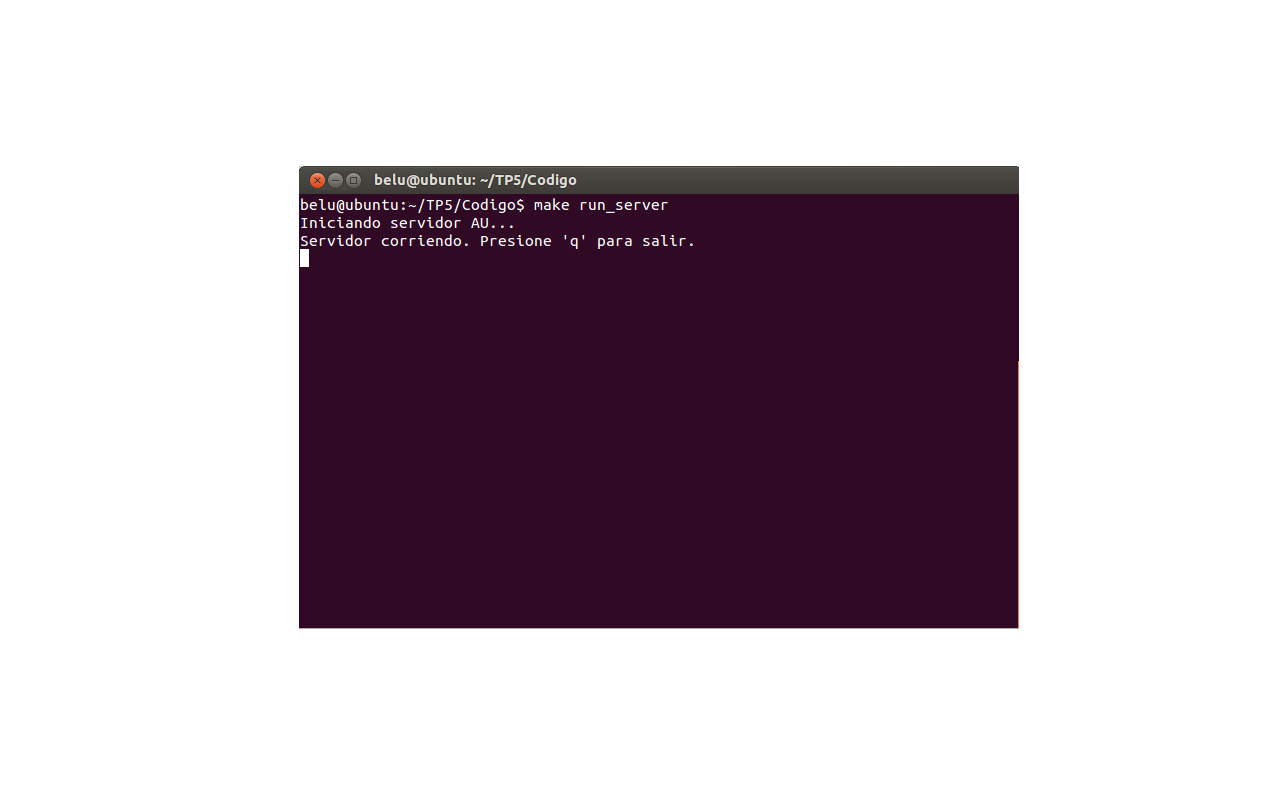
\includegraphics[width=0.85\textwidth]{Server.png}
	\bigskip
       \caption{Consola del server.}
	\end{figure}

\subsection{Aplicación Monitor}
\smallskip
	Al ejecutar la aplicación monitor, se observa una pantalla de inicio de sesión en la que se debe ingresar el nombre ADMMONITOR y la clave 'admin1234'. Alli, se inicia la comunicación entre el servidor (que debe estar corriendo) y el monitor.
	\begin{figure}[h]
       \centering
       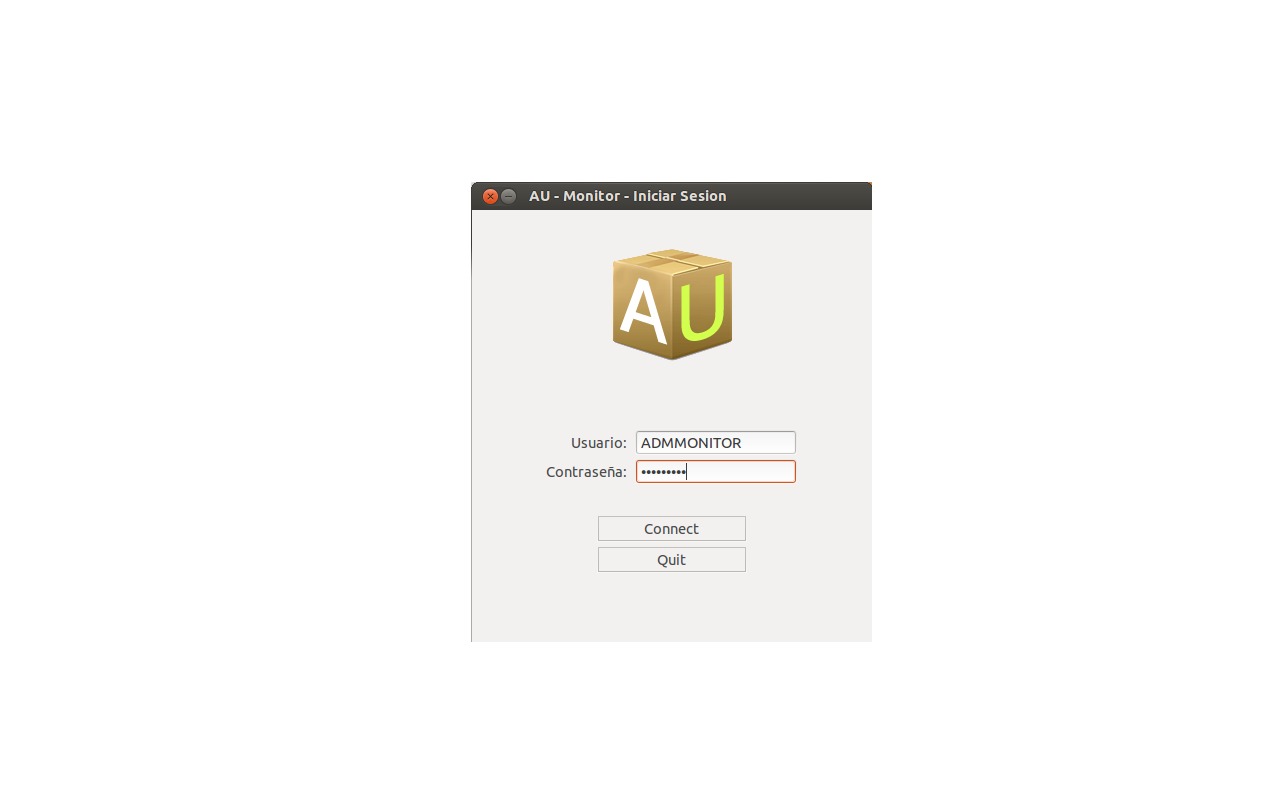
\includegraphics[width=0.85\textwidth]{InicioMonitor.png}
	\bigskip
       \caption{Inicio de sesion del monitor.}
	\end{figure}
	Luego de iniciar sesión correctamente, se accede a una pantalla donde se pueden observar menu de opciones.
	\begin{figure}[h]
       \centering
       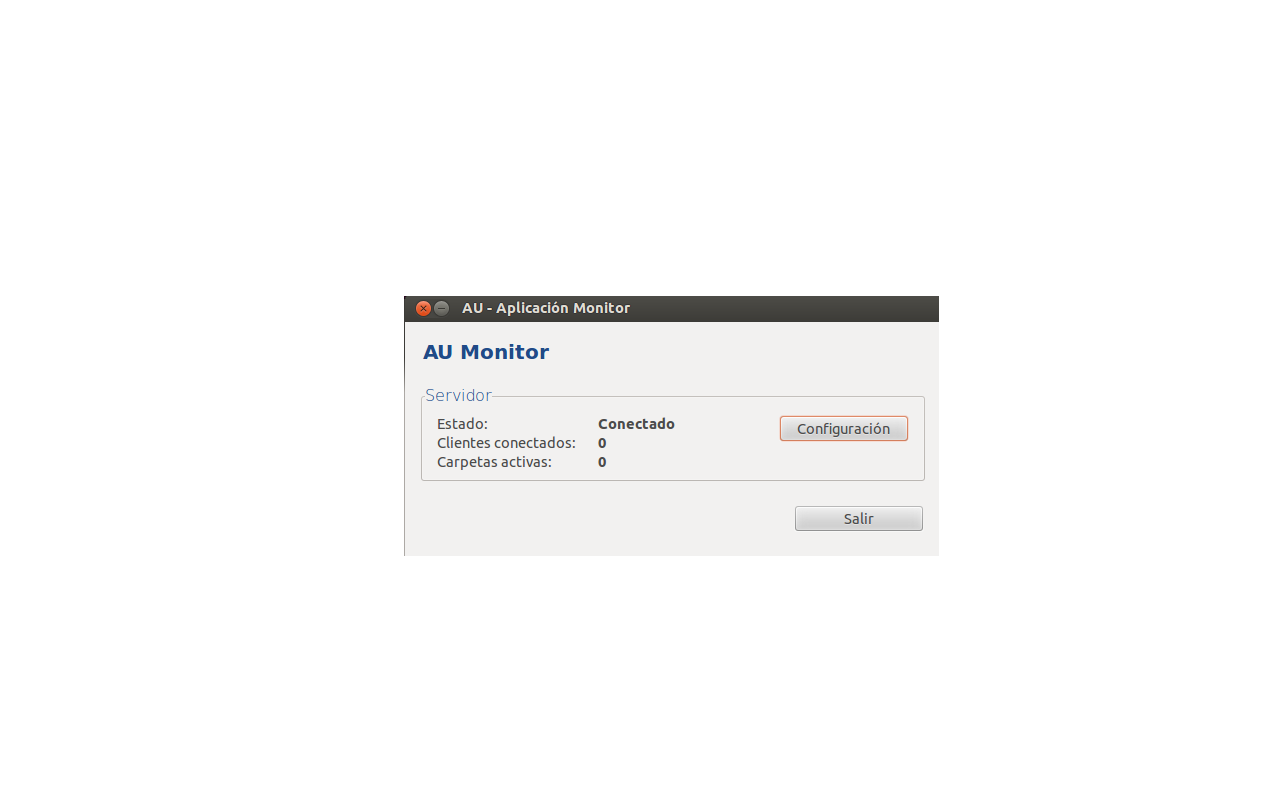
\includegraphics[width=0.85\textwidth]{MonitorPPal.png}
	\bigskip
       \caption{Vista inicial del monitor.}
	\end{figure}
	Desde la opción \textit{Administrar Usuarios}, se pueden administrar las cuentas de todos los usuarios registrados o por registar. Se pueden ingresar nuevos clientes, utilizando el boton \textit{Agregar Usuario}. De aquí, se pasa a una ventana en donde se debe ingresar 'Nombre de usuario' y 'Contraseña'. Para guardar los cambios, presionar 'Guardar'.
	\begin{figure}[h]
       \centering
       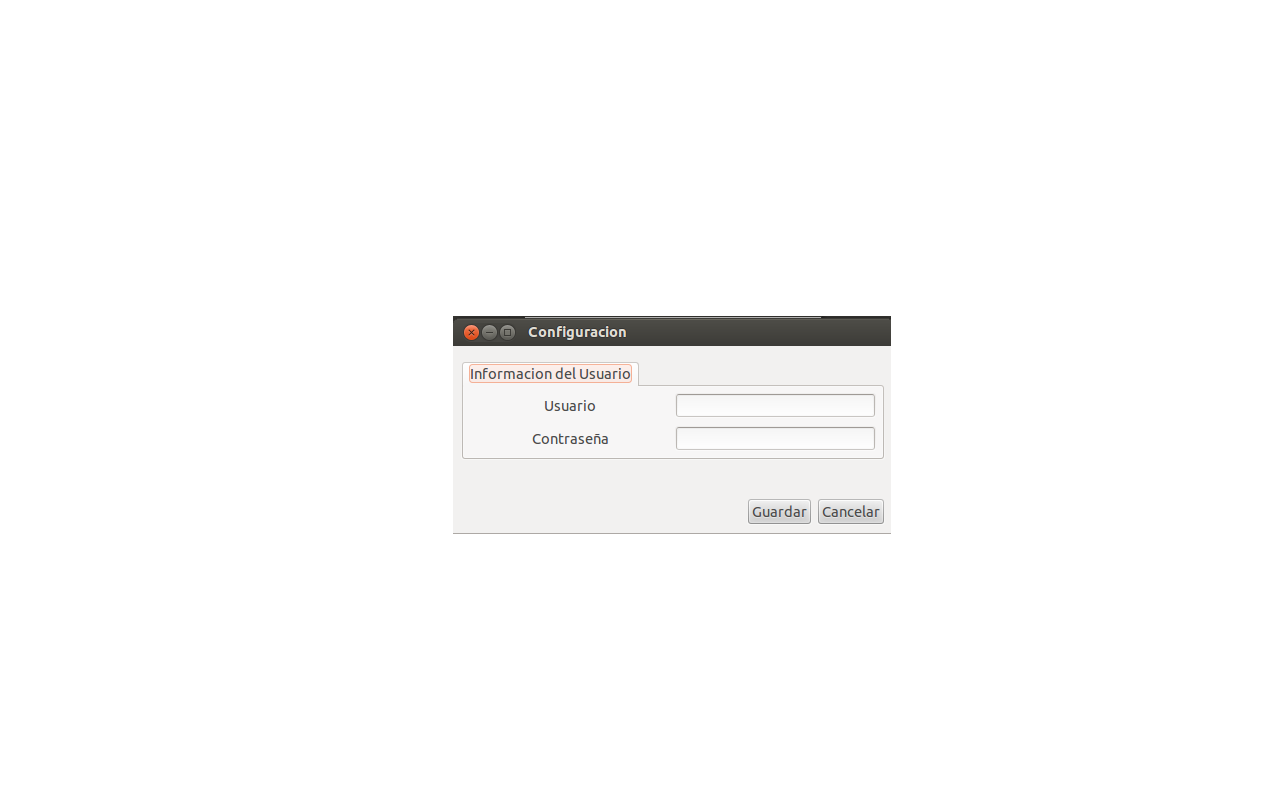
\includegraphics[width=0.85\textwidth]{NuevoUsuario.png}
	\bigskip
       \caption{Interfaz de nuevo usuario.}
	\end{figure}
	Para modificar usuarios existentes, se debe seleccionar uno de la lista y presionar el boton \textit{Modificar Usuario}. Solamente se podrá modificar la clave asociada al usuario que se seleccionó.
	\begin{figure}[h]
       \centering
       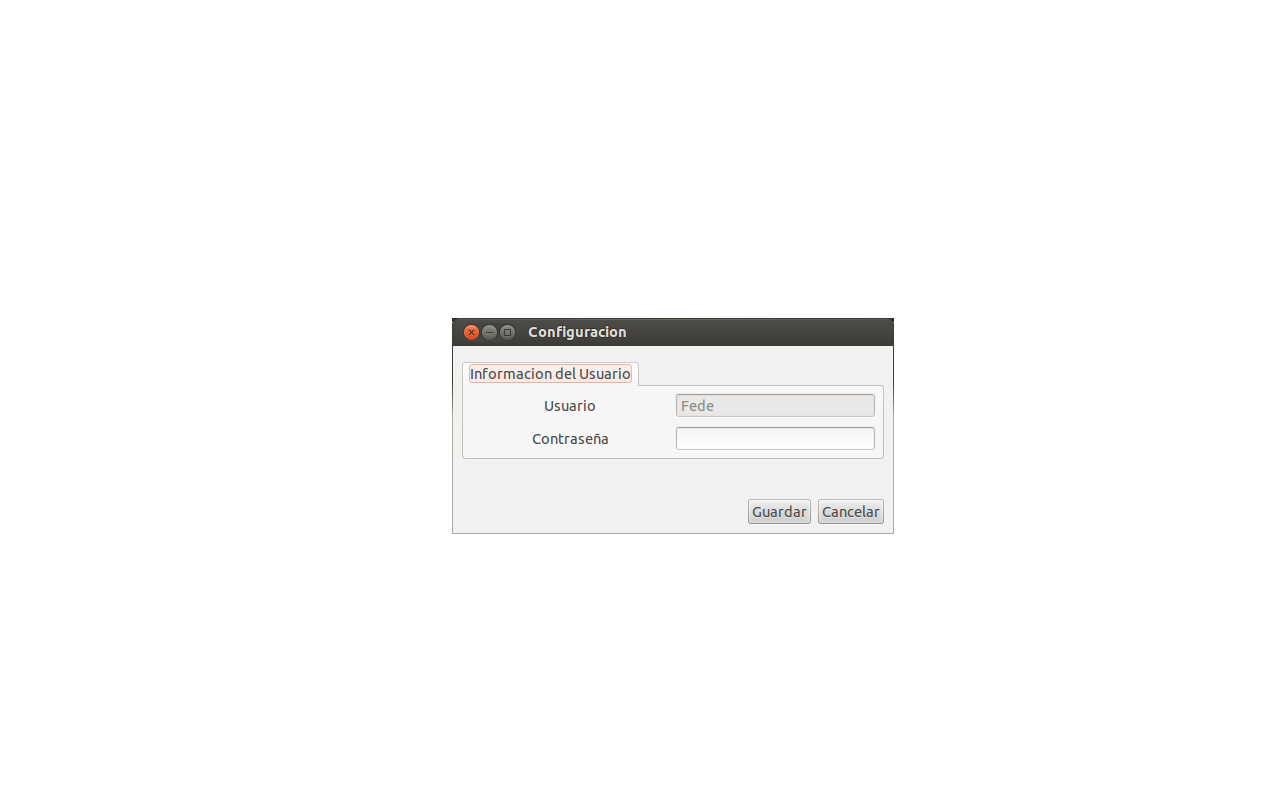
\includegraphics[width=0.85\textwidth]{ModifUsuario.png}
	\bigskip
       \caption{Interfaz de modificar usuario.}
	\end{figure}
	Luego, se podrá eliminar un usuario existente, seleccionandolo de la lista y presionando el boton \textit{Eliminar Usuario}. Se abre una ventana preguntando si realmente desea eliminarlo.
	\begin{figure}[h]
       \centering
       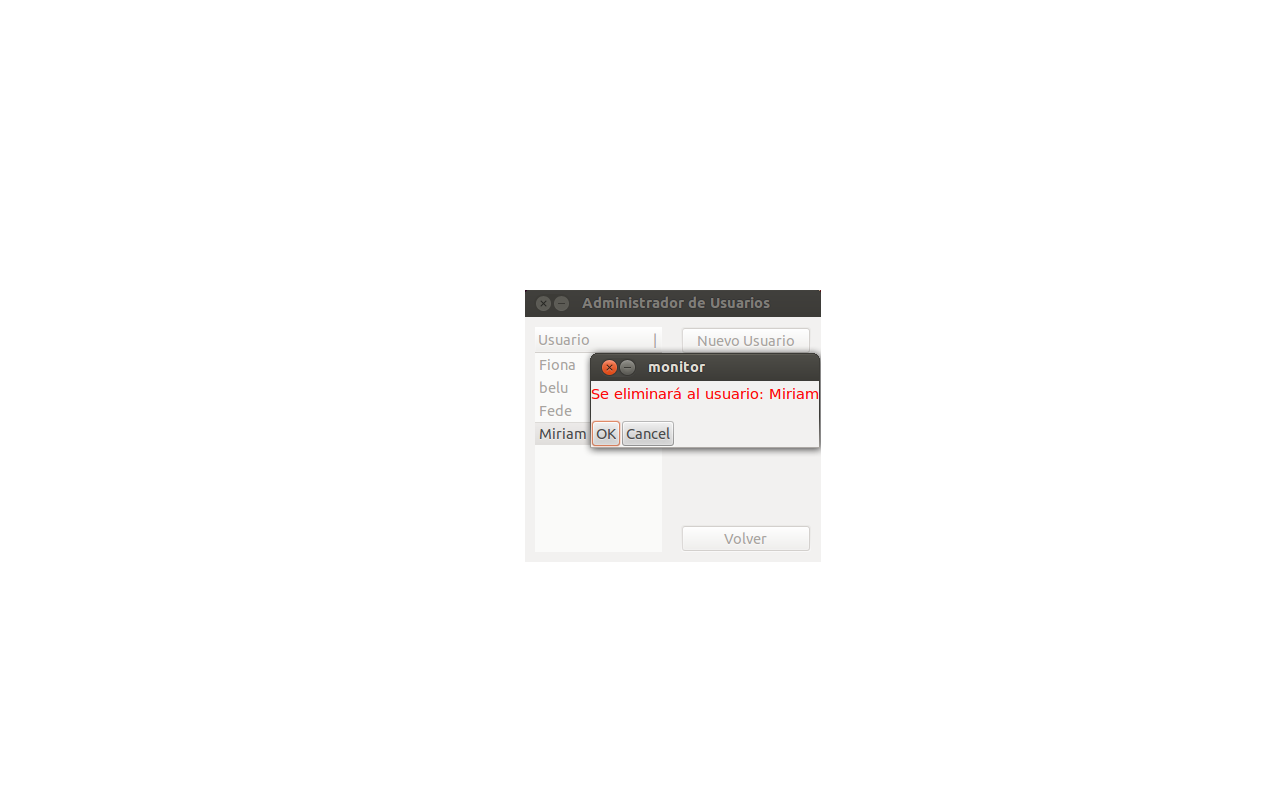
\includegraphics[width=0.85\textwidth]{EliminarUsuario.png}
	\bigskip
       \caption{Eliminar Usuario.}
	\end{figure}
	Finalmente, se puede acceder a una sección de configuración del Monitor, donde se puede especificar por ejemplo, el puerto utilizado.
	\begin{figure}[h]
       \centering
       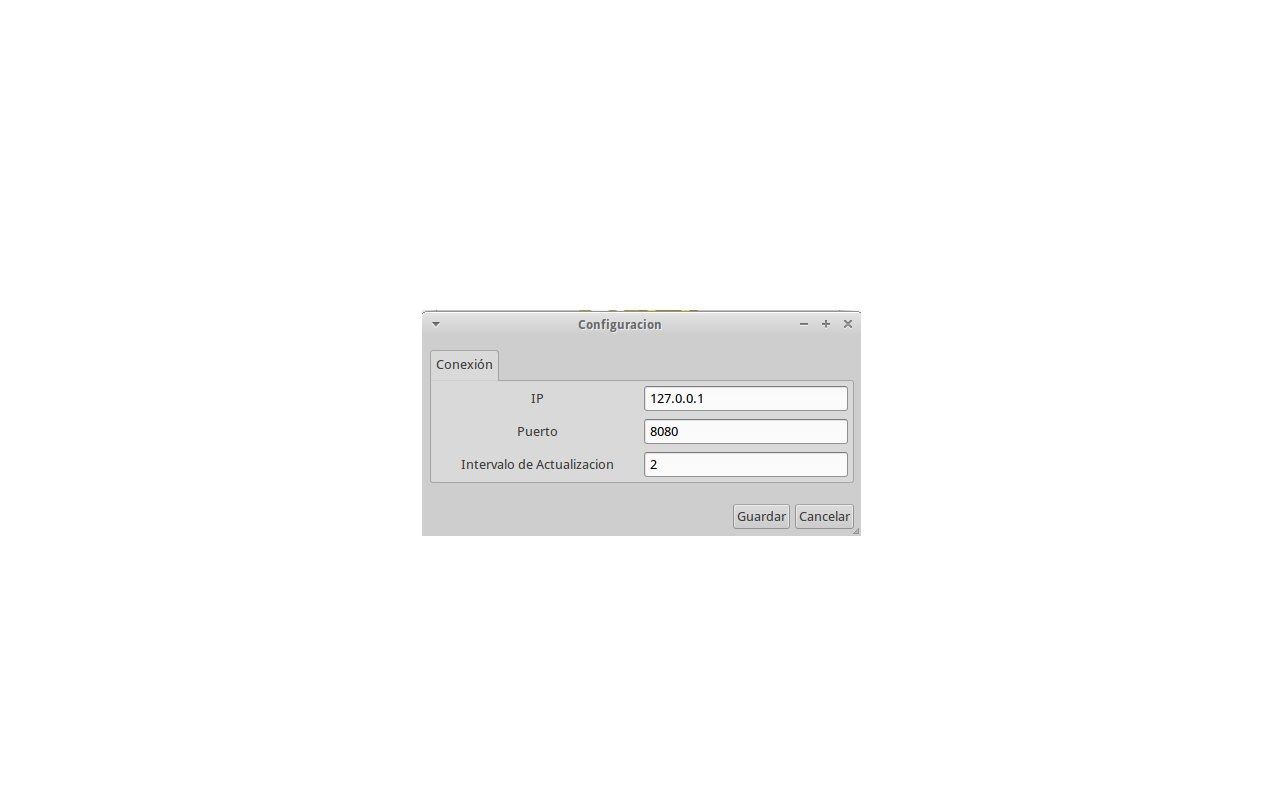
\includegraphics[width=0.85\textwidth]{configuracionMonitor.png}
	\bigskip
       \caption{Configuración del monitor.}
	\end{figure}

\subsection{Aplicación Cliente}
\smallskip
	Al ejecutar la aplicación cliente, se observara una pantalla de inicio de sesión en la que se debe ingresar el nombre de usuario y contraseña. 
	\begin{figure}[h]
       \centering
       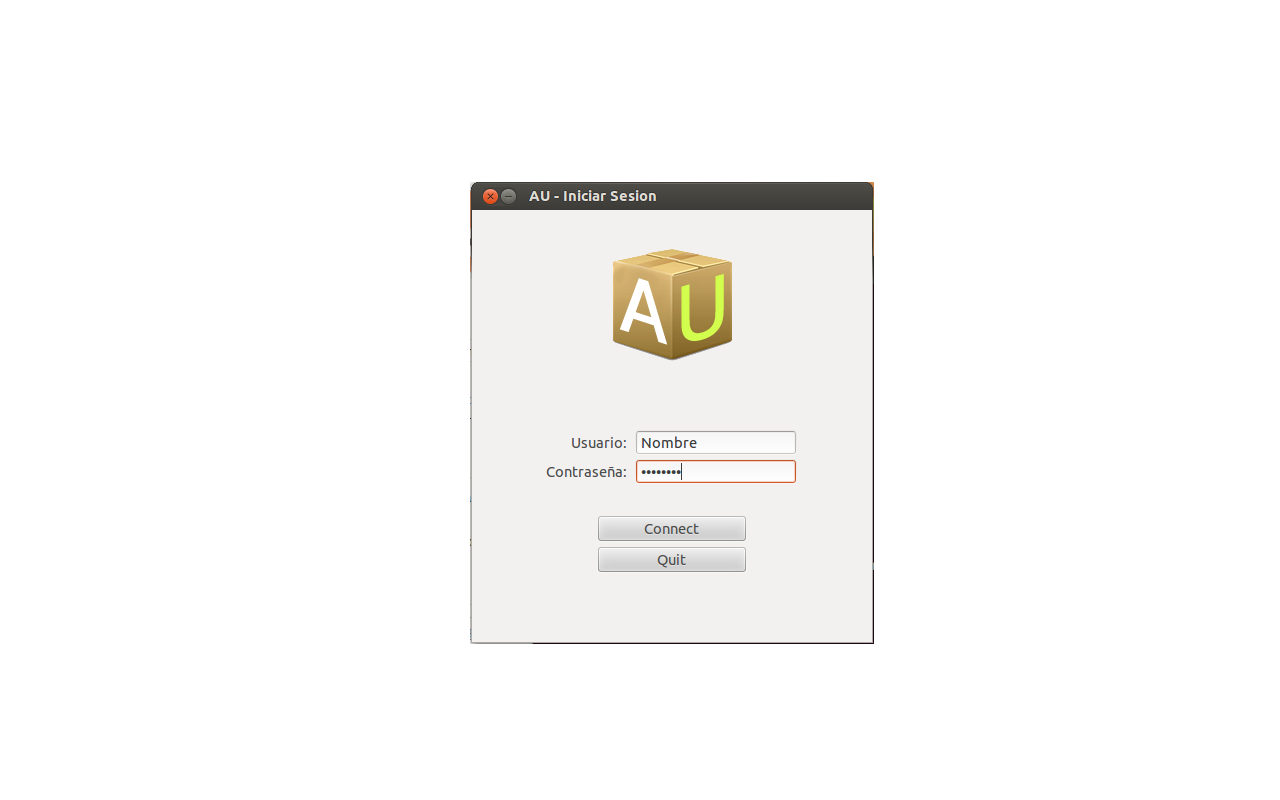
\includegraphics[width=0.85\textwidth]{InicioSesionCli.png}
	\bigskip
       \caption{Inicio de sesion de cliente.}
	\end{figure}
	Se pueden modificar las opciones en la aplicación, obteniendo una ventana de Preferencias. Aquí, se pueden modificar el directorio que se quiere sincronizar, la IP del servidor al cual se quiere conectar y además el puerto (de estar loggeado, no se podrán modificar ninguna de estas dos últimas).
	\begin{figure}[h]
       \centering
       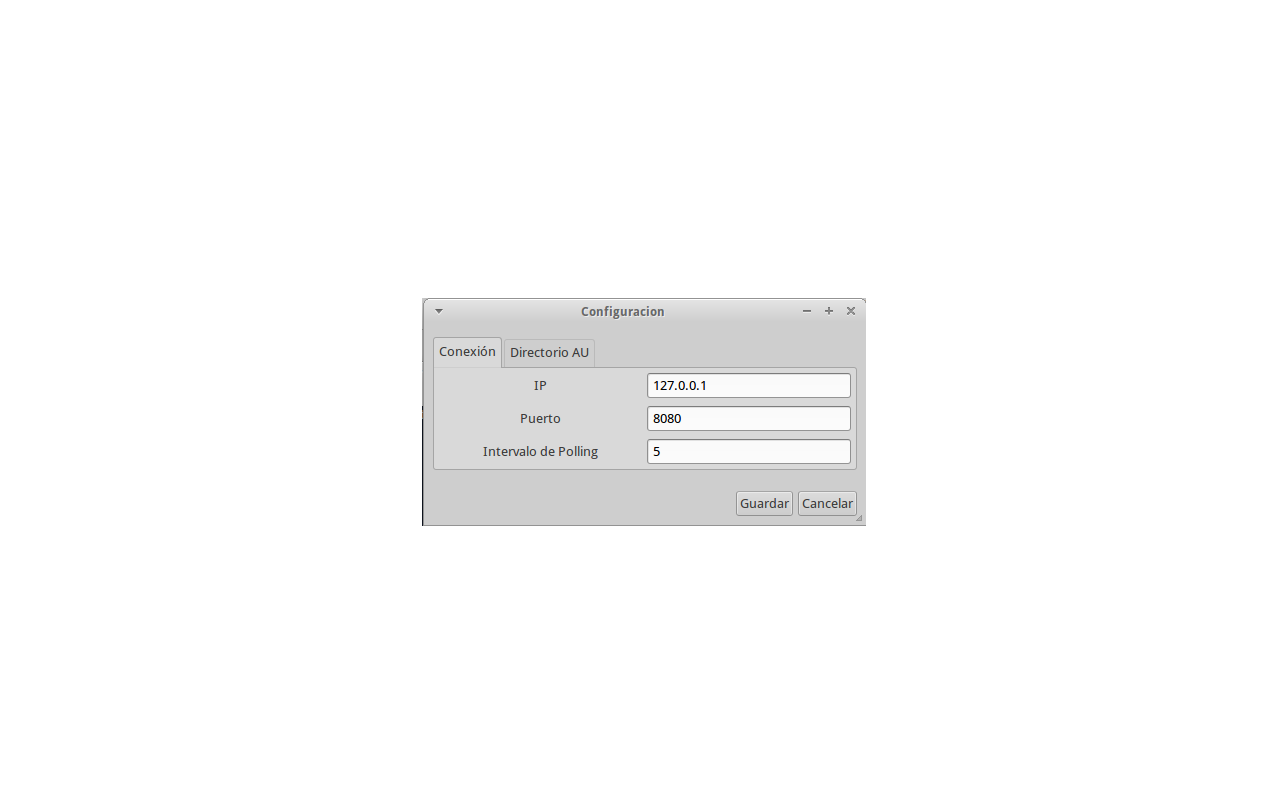
\includegraphics[width=0.85\textwidth]{configuracionCliente.png}
	\bigskip
       \caption{Configuración de cliente antes de log in.}
	\begin{figure}[h]
       \centering
       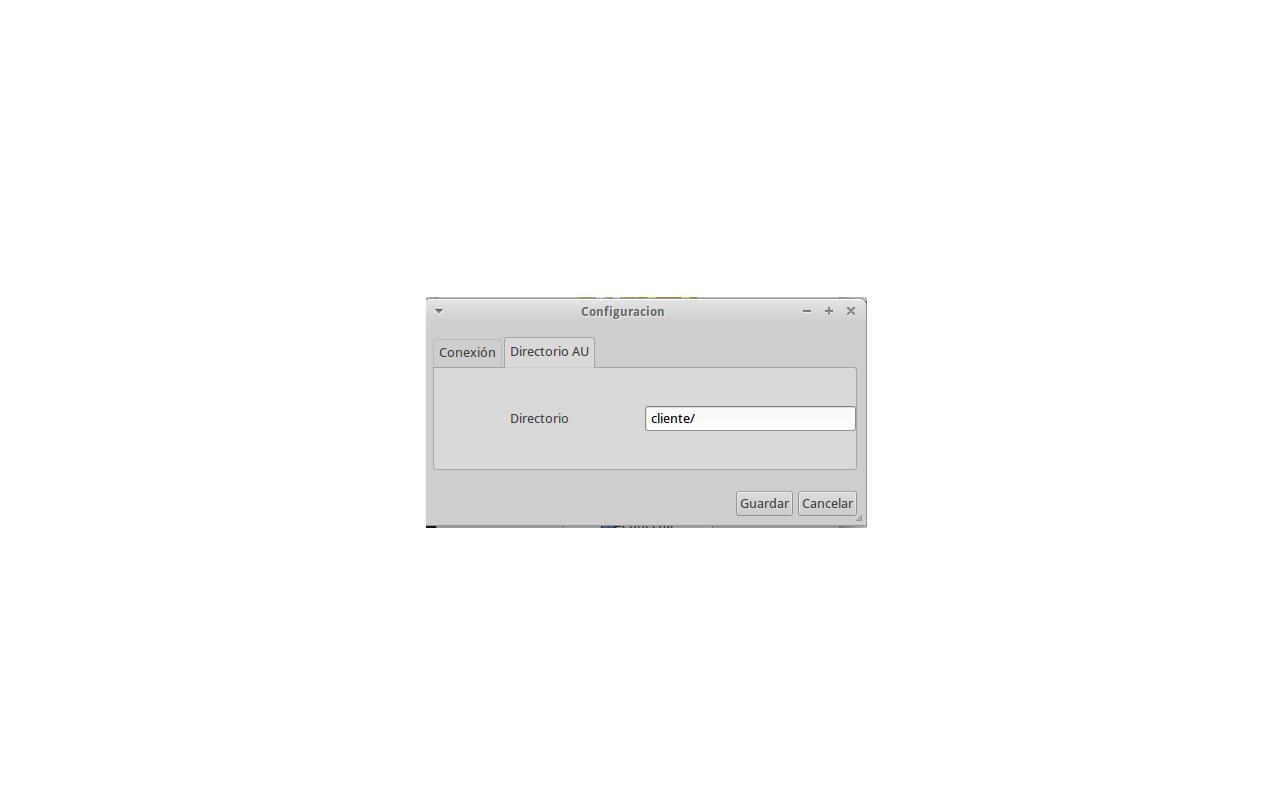
\includegraphics[width=0.85\textwidth]{configuracionCliente2.png}
	\bigskip
       \caption{Configuración de cliente luego de log in.}
	\end{figure}
	Luego, al entrar en el proceso de sincronización, se entra en una pantalla de sincronización.
	\begin{figure}[h]
       \centering
       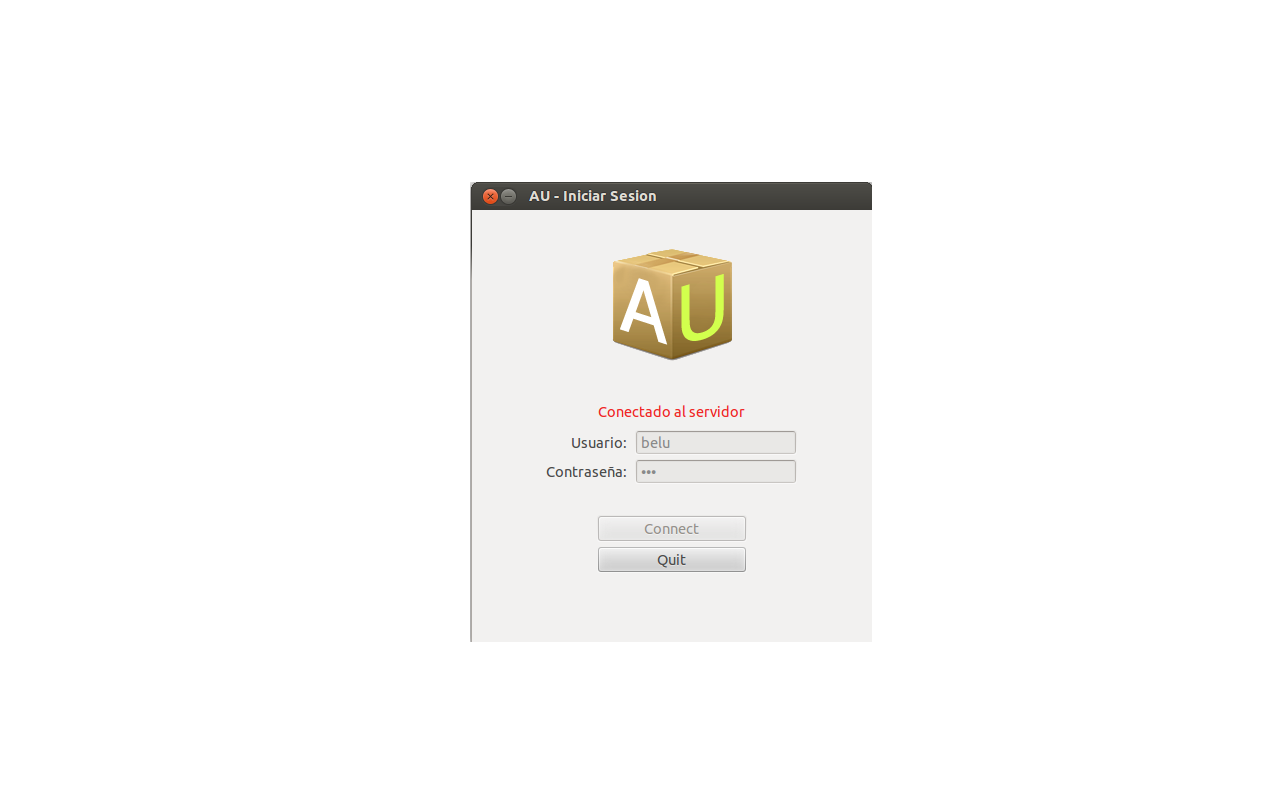
\includegraphics[width=0.85\textwidth]{Sincronizando.png}
	\bigskip
       \caption{Sincronizacion.}
	\end{figure}
\bigskip




% APENDICE DE ERRORES
\section{Apéndice de errores}
	
	A continuación se provee una lista de posibles errores que pueden obtenerse durante la ejecución de la aplicación:
	\par
Errores en conexión:
\begin{itemize}
\item "ERROR: No se ha podido cerrar el socket." : Se obtiene este error si no se logro cerrar correctamente el socket.
\item "ERROR: No se ha podido crear el socket." : Se obtiene este error si no logra crearse el socket correctamente.
\item "ERROR: No se pudo llevar a cabo la conexión." : No se logró conectar el cliente al socket destino.
\item "ERROR: No se pudo comenzar a escuchar." : El socket del servidor no logro crearse correctamente.
\item "ERROR: No se pudo aceptar la conexión" : El socket del servidor no logró aceptar una nueva conexión.
\item "ERROR: Antes de enlazar, no se pudo reutilizar socket." : Si cayó la conexión inesperadamente y no se pudo reestablecer la conexión en el mismo puerto, se obtiene este error.
\item "ERROR: No se pudo llevar a cabo el enlace." : El servidor no se pudo enlazar correctamente a un puerto. Puede ser que este puerto ya esté en uso por alguna otra aplicación.
\end{itemize}

	\par
Errores en manejo de archivos:
\begin{itemize}
\item "ERROR: Archivo de entrada inválido." : Este error se obtiene cuando se está intentando acceder a un archivo que no pudo ser abierto. Puede ser que ya no exista en disco o que esté en uso por otra aplicación.
\item "ERROR: El archivo no pudo ser abierto." : idem anterior.
\item "ERROR: El registro no pudo ser abierto." : Este error se puede obtener cuando el archivo \textit{.reg_archivos} no logró ser abierto correctamente.
\item "ERROR: No se ha podido abrir el directorio." : Este error se puede dar cuando el directorio está protegido o no existe la ruta de directorio especificada.
\item "ERROR: Archivo nuevo no pudo ser creado." : Este error se obtiene cuando no se pudo crear un archivo nuevo. Puede suceder, por ejemplo, que no se tiene más espacio en disco. 

\end{itemize}
\bigskip



\end{document}
